\renewcommand{\glyph}{\iconfont{\XeTeXglyph292}}
\chapter{Conclusion} \label{chapter6}
\minitoc
\eject

The web brought a new economic model allowing a tremendous number of business opportunities.
To seize these opportunities, a team needs to develop a web application, and grow a business around it.
The economical incentives around the technical development changes completely during the growth of this business.
In the beginning, the development needs to be productive, to quickly release a product and iterate with the user feedbacks.
When the project matures, the execution needs to be efficient, to cope with the load of a large user base while limiting the hardware costs.

These two development concerns are incompatible.
No platform can provide both performance efficiency, and development productivity at the same time.
The platforms at the state of the art propose only compromises between the two.
This thesis presented a platform allowing a progressive compromise to fit the economical incentives throughout the evolution of the project.

This chapter summarizes the contributions of this thesis, and evaluates the proposed solution.
It finally concludes on the perspectives beyond this thesis.

\section{Summary} \label{chapter6:summary}

This thesis presented an equivalence between the event-driven execution model and the pipeline execution model.
This equivalence was implemented into two compilers.
The first compiler allows to identify the rupture point to form chains of stages from programs targeting the event-driven execution model.
The resulting chains still depends on a common memory store.
The second compiler, stemming from the first one, identifies the entry points of these chains - start rupture points - and enforces isolation to form a parallel pipeline.

With these two contributions, it is possible to transform the modular representation of an application into a pipeline representation.
The modular representation allows development productivity, while the pipeline representation executes efficiently.
A development team shall then use these two representations to continuously iterate over the implementation of an application, and reach the best compromise between productivity and efficiency.

The next paragraphs summarizes the two execution models, and the steps of this equivalence from one model to the other.

\subsection{Models} \label{chapter7:summary:model}

\paragraph{Event-driven execution model}

The event-driven execution model is targeted by productive programming languages.
It processes a queue of asynchronous events by scheduling handlers cooperatively.
Each handler can asynchronously request resources and define handlers to receive the resource response. 
The handlers are chained by these asynchronous requests using continuation passing style.
Apart from the resource response, the communication between tow handlers is done via closures.
The downstream handler gets access to the environment of its creation through a closure.

They are organized similarly to a pipeline, each handler being a stage, with the data flowing from one stage to the other.
However, the handlers still share a common memory store.
It allows the higher-order programming required for productivity.
But it also avoids the parallelism required for efficiency.

\begin{figure}
  \centering
  \textfig{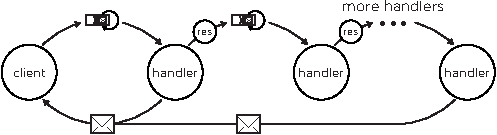
\includegraphics[width=0.8\linewidth]{../resources/cont-chain.pdf}}
\end{figure}

\paragraph{Fluxional execution model}

The fluxional execution model is targeted by a more efficient programming language.
It executes an application expressed as a network of independent application parts called fluxions.
The fluxions communicate by messages, and form a pipeline similarly to the handlers of the event-driven execution model.
They are executed in parallel to distribute the computation across several cores and increase the performance efficiency.
They rely on isolated memory store, called context to allow this parallel execution.
When several fluxions need to rely on the same memory store, they are grouped, and executed sequentially.
When they are independent, they are isolated to increase performance efficiency.

The similarity between the event-driven execution model and the fluxional execution model leads to the equivalence presented in the next paragraph.
With this equivalence, the versatility of fluxions allows to progressively adapt the implementation from a productive, single event-loop, toward an efficient pipeline.

\subsection{Equivalence}

The equivalence describes the transformation from an application targeting the event-driven execution model to execute them in parallel in the fluxional execution model.
This transformation involves two steps: the extraction and isolation of the stages to form the pipeline.

\paragraph{Stage Extraction} \label{chapter7:summary:extraction}

The first step is the identification and extraction of the stages.
The equivalence identifies rupture points between stages.
A rupture point is an asynchronous call without subsequent synchronization with the caller.
It indicates a rupture in the synchronous control-flow, and the boundaries between two handlers.
The upstream handler is the one calling the asynchronous call, the downstream handler is the callback provided to the asynchronous call.

There are two kinds of rupture points: \textit{start} and \textit{post}.
\textit{Start} rupture points directly receives the input stream, and start the execution of the chain of stages for each new datum in the stream.
\textit{Post} rupture points indicates a continuity in the chain of stages.

The difficulty in this compilation step is to identify the asynchronous functions indicating the stages.
Because of the dynamic behaviors of Javascript, it is impossible to statically detect these functions.
The compiler implemented from the equivalence is currently unable to reliably detect them.
Instead the compiler rely on the developer to provide a list of asynchronous function names to extract.

\paragraph{Stage Isolation} \label{chapter7:summary:isolation}

% After the extraction of this pipeline,
The second step is the identification of the memory interdependencies between stages.
It intends to isolate the stages so they can be executed in parallel.
The common memory is replaced by message-passing, following some rules to preserve consistency.
\begin{itemize}
\item If a stage needs to hold a variable from one request to the other, this variable is stored in its context.
\item If a downstream stage needs to read a variable from an upstream stage, the variable is sent as part of the message communication.
\item If two stages needs to share a variable, they are grouped on the same execution node to safely share parts of their context.
Their executions are not parallelized to avoid conflicting accesses.
\end{itemize}

The difficulty in this step is to identify the memory dependencies between stages.
The dynamic behaviors of Javascript, it is impossible to statically identify the aliasing in the memory.
The compiler implemented from the equivalence is currently unable identify these interdependencies.
It relies on manual manipulations to complete the transformation.

\separator

These difficulties are details in further details in the next section.
It then presents some perspectives to overcome these limitations.
\section{Overall Evaluation} \label{chapter6:evaluation}

The equivalence presented in chapter \ref{chapter4} is implemented in a the fluxional compiler, presented in section \ref{chapter5:flx}.
This implementation is evaluated against the criteria presented in chapter \ref{chapter3}, Productivity, Efficiency and Adoption.

\subsection{Trading Productivity for Efficiency}

% \subsubsection{Productivity}

The equivalence intends to disrupt as less as possible the way developer build web applications.
The goal is to avoid degrading the productivity, hence the adoption, of the proposed platform.
% The source language, Javascript, is left intact, except for the forbidden statements \texttt{with} and \texttt{eval}.
% These statements are already forbidden by some good practice guides \cite{Crockford2008}.
Therefore, the productivity is intended to be the same as the original event-driven platform.

However, in the current state, the compiler implementation is unable to operate the transformation without an external help.
The static analysis is unable to correctly detect the aliasing of the memory in Javascript.
It avoids developers to use Higher-Order Programming, hence impacts composition.
This limitation avoids to improve the current trade-off of productivity for efficiency, as illustrated in table \ref{tab:proposition-productivity}.
Indeed, to gain efficiency, developers need to commit efforts to indicate the stages of the pipeline, and assure their dependency.

% \TablePropositionProductivity{tab:proposition-productivity}

The manual transformation process yields a distributed application, similarly as the other efficient platforms.
And the chapter \ref{chapter3} showed that such applications achieve very good performance efficiency.
But the productivity limitation remains.
It avoids the current implementation to propose a satisfying compromise between productivity and efficiency.
So, the current implementation actually trades productivity for efficiency, similarly to many platform in the state of the art. % , as illustrated in table \ref{tab:proposition-efficiency}.
The perspectives to overcome this limitation are addressed later in section \ref{chapter5:evaluation:perspective}.
% \TablePropositionEfficiency{tab:proposition-efficiency}


% It doesn't make any sense to evaluate an application, as the transformation would not reflect the compilation process, but the manual transformation process.

% If the runtime memory analysis is solid enough to detect correctly the aliasing of the memory, then it will be able to help the development team transitioning from productivity to efficiency, which is the response of this thesis to the problematic.

\subsection{Adoption}

As observed in the chapter \ref{chapter3}, trading productivity for efficiency drastically reduces adoption.
Because the current implementation presents the same limitation than the efficient platforms, its adoption is not expected to be different. %, as illustrated in table \ref{tab:proposition-adoption}.

Yet, both productivity and efficiency are required for the platform to be adopted by new developers as well as large businesses.
Only at this condition, will it reinforce the loop between community and industry.
So the current implementation is not expected to be widely adopted, as presented in the table \ref{tab:proposition-summary}.

\TablePropositionSummary{tab:proposition-summary}
% \TablePropositionAdoption{tab:proposition-adoption}

% It was briefly tested during the development of the grumpy application, presented in chapter \ref{chapter4}, section \ref{chapter4:execution-models:examples}.

The limitation of static analysis avoids the equivalence to be fully implemented to address the problematic.
Hence, this evaluation holds only on the implementation, and not on the equivalence.


When saying that \textit{it is a mistake to attempt high concurrency without help from the compiler}, R. von Behren \textit{et al.} \cite{Behren2003} implies that the language alone cannot achieve high concurrency.
It is necessary to rely on additional tools, such as a compiler to reach the best compromise between productivity and efficiency.
The evaluation of this thesis concludes that static analysis is unable to reach this compromise for the current multi-paradigm languages using higher-order programming.
% Before dropping all higher-order languages for the sake of efficiency,
Yet, there exist alternatives to static analysis to reach this compromise.
The next paragraph presents some interesting perspectives of this work to further address this problematic.

% In the contribution of this thesis, the two main difficulties, identifying stages and detecting memory dependencies, are due to the dynamic nature of Javascript.
% A perspective to overcome these limitation is to implement the transformation, not as a compiler, but as a runtime.
% Indeed, at runtime, all the dynamic behavior are resolved, and the analysis can be much more precise, and less speculative.

% \subsection{Fluxionnal Runtime} 

% \section{Perspectives}

% Javascript is a highly dynamic languages.
\section{Perspectives} \label{chapter6:perspective}

As stated previously, static analysis impacts productivity to favor efficiency.
% For example, to isolate fluxions, the current implementation of the compiler restrains the developer to use only \textit{in situ} callbacks, and avoids aliasing.
Though, an interesting perspective to continue this work is to implement the equivalence as a just-in-time compiler.
Indeed, the dynamic analysis allowed at run time is more prone to overcome the limitation identified with static analysis.

\subsection{Just-in-time Compilation}

Most Javascript interpreters compile some parts of the code at run time to improve performances.
During this compilation, the levels of indirections are mostly resolved.
The code is translated directly into lower-level instructions.

Implementing the equivalence in a just-in-time (JIT) compiler could leverage this dynamic resolution.
It could analyze the scope of variables resolved dynamically, and isolate the stages accordingly.

\paragraph{Rupture point detection}

The asynchronous functions identifying rupture points are not part of Javascript.
They are special functions provided by the interpreter.
With the compiler communicating with the interpreter at run time, detecting rupture points become trivial.
The interpreter notifies the compiler when an asynchronous function is called.
The compiler then identifies the rupture point and isolates it to possibly execute it remotely.

\paragraph{Dominator Tree}

To debug the memory in dynamic languages like Javascript, one can use a dominator tree.
It is a tree generated at run time indicating the parenting relations between memory objects.
With such a tree, the analysis of interdependencies between stages becomes trivial.
Each stage can be isolated in a fluxion, and deployed accordingly to its dependencies.

% With the dynamic registering of Fluxions to the messaging system, and into tag groups, it is possible to transform a Javascript application continuously during its execution.
% Analysis of the interdependencies become as trivial as for static languages, with the resolution of the indirections by the just-in-time compiler.
% The fluxional compiler waits for these resolutions, and then analyzes the compiled code for rupture points.
% As the asynchronism of a function call is handled by the execution engine, the just-in-time compilation can pin point precisely the asynchronous calls from the synchronous ones. 
% And the continuations for these asynchronous calls are resolved, which makes them similar to inline continuations.

\paragraph{Closure Serialization}

Closures are required to allow higher-order programming.
But the static compiler is unable to manipulate closures, as illustrated in section \ref{chapter5:flx:evaluation:isolation}.
Closures are generated dynamically by the interpreter.
With the compiler communicating with the interpreter, the former can manipulates and serialize them at run time.
It can then send closures between fluxions, like any other objects.
It enables the use of higher-order programming within the fluxional execution model.
Hence, it would allow, to some extent, to improve the compromise between productivity and efficiency.
Indeed, the developer is free to use the higher-order programming to compose modules, with a global memory abstraction.
Yet, the execution could distribute this global memory abstraction according to the detected interdependencies.

\paragraph{Dynamic Grouping}

With the dynamic detection of stages and their dependencies, and the manipulation of closures, fluxions can be registered during the execution of the application.
To assure they meet their dependencies, the fluxions are deployed according to their groups.
Two fluxions belong to the same group if they need to share access to some variables.
Therefore, they need to be deployed on the same event-loop to share their memory.

\paragraph{Safe-Checking}

It is required to safe-check that the compiled code is consistent with the remaining execution.
As an example, just-in-time compilers check the type to assure that a compiled function remains conform to the input and output types of its call site.
Similarly, it is required to check that the deployment of fluxions doesn't cause inconsistencies.

If a fluxion ready to be deployed belongs to two different groups, these two groups needs to be gathered on the same event-loop.
If they were previously deployed on two different event-loops, they need to be moved with their context to be on the same event-loop.
Moreover, to assure consistency, they need to be moved when receiving the request that triggered the fluxion ready to be deployed.
So that when this new fluxion is executed at this message reception it has access to the contexts of the two groups.
For this purpose, the compiler put the execution on hold, and sends a control message downstream to order the move of the fluxions.
% It interleaves control messages in the stream to communicate with the distributed interpreters.
In this example, the message inquired the distributed interpreters to stop execution, pack the fluxions and their contexts, and send them back to another remote interpreter.
To assure consistency, the execution resumes only when all the fluxions are gathered in the same event-loop, with access to the whole shared memory.

% If the new fluxion depends an a local variable, as well as a variable from a group on another node than the local node, the group needs to be deployed back locally.
% The fluxion as well as all the fluxions of the group are deployed locally, but the execution needs to wait for the contexts of the group to be available locally.
% To gather the contexts, the node responsible for this group send a message to the messaging system managing this group.
% The messaging system gather all the contexts of the fluxions, and send them back.
% When the contexts are deployed locally to the new node responsible for the this group, the execution of this branch can resume.

% A new compromise have to be done between the cost of sending a fluxion and the cost to get it back, and the risk that it requires to be sent back.
% It might be possible to reduce this risk by saving the compilation information from one execution to the other.

\separator

The perspectives described in the previous paragraphs overcome the limitations of the current implementation of the compiler.
They describe the further implementation of the equivalence, as if I were to continue this work.

\subsection{Evaluation of the perspective}

This second evaluation admits that the JIT compilation resolves all the indirections in the memory.
% Which is left unknown after this thesis.
Then, the fluxional JIT compiler doesn't need to rely on human interaction.
Therefore, the expected productivity is the same as the productivity language used as source. %, as illustrated in table \ref{tab:perspective-productivity}.

% \TablePerspectiveProductivity{tab:perspective-productivity}

Naturally, the performance efficiency of the implementation is, at first, the same of this productivity language, as the development is focused on productivity.
Some development efforts are required to improve the efficiency.
% But the result of the compilation helps in this shift.
The result from the compiler helps the developer find the bottle necks, and reduce the effort for this shift.
With the help from the compiler, the effort for this shift is expected to be less than the current required effort.
% The effort for this shift are expected to be less than the current required effort. %, as illustrated in table \ref{tab:perspective-efficiency}.
Instead of redesigning the architecture of the application to immediately isolate components, it is possible to modify them to progressively loosen their dependencies.
As illustrated in table \ref{tab:perspective-summary}, this envisioned platform is expected to yield both productivity and efficiency, not at the same time, but when they are required the most.

% \TablePerspectiveEfficiency{tab:perspective-efficiency}

Moreover, during this decomposition and after, developers can still rely on higher-order programming, even between isolated application parts.
In the current state of the art, there is no known platform to offer higher-order programming between distributed parts.
This possibility is therefore unknown, and could actually yield to an unrivaled compromise between productivity and efficiency.

Following the insight along this thesis, a platform bringing both productivity and efficiency simultaneously would be greatly adopted.
But it requires to be observed in real conditions before drawing this conclusion.
% , as illustrated in table \ref{tab:perspective-adoption}.

% \TablePerspectiveAdoption{tab:perspective-adoption}
% \separator

\TablePerspectiveSummary{tab:perspective-summary}

\subsection{Final Thoughts}

During this thesis, I progressively changed my vision of our everyday world.
As a final note in this thesis, for what it is worth, I would like to share this vision I believe to be atypical.

% \paragraph{Economic Considerations}

Nearly 3 decades ago, the IT industry understood that trading efficiency for productivity could reduce development time and thus, the final cost.
Hardware performance could compensate the loss of execution efficiency.
But the new challenge to build available web services at a world wide scale requires efficiency again.
Moreover, the IT industry has an important impact on the ecology with its increasing carbon footprint.
As explained all along this thesis, I believe that it is time to take into account both productivity and efficiency.
% As the digitalization permeates into every aspects of our lives, it is of crucial importance to consider this impact.

Yet, programming cannot be reserved to experts anymore.
As digitalization permeates into every aspects of our lives, it is of crucial importance that programming be available for everyone.
Productivity cannot be traded back for efficiency.
This thesis intends to bring a modest reconciliation between two economical concerns for a web application, the efficiency of execution and the productivity of development.
But it still feels like developers are an elite, and are comparable to the copyist monks before the invention of printing.

Internet disrupted the way we learn and share knowledge.
In this continuity, I believe that in the time to come, programming will be mastered by everybody.
Additionally as reading and writing, developing will be a prerequisite to communicate with peers.
For example, it will allow to express dynamic behaviors, and not only static ones, as Bret Viktor already envisioned\ftnt{https://vimeo.com/115154289}.
I believe that this shift will disrupt the way to see, live and interact with our surroundings and with peers.
A way we could barely imagine today.
% One objective I see for the regulation of system is the scalability of said systems.

Yet, some examples show that this shift might actually already be happening.
The platforms Squarespace\ftnt{http://www.squarespace.com/} and the soon to come Grid\ftnt{https://thegrid.io/} allow everyone to launch a commercial store front on the web without any required programming knowledge.
It illustrates well that technology is bound to be at the service of social evolution, and not be an unreachable field reserved to academics.

This shift of communication might come with the increasing importance of machine learning and artificial intelligence.
Similarly to programming, it allows to easily define complex behaviors.
% Machine learning  without specifically describing every corner cases
% It feels like the composition of general behaviors can seamlessly meld at corner cases.
I use the following metaphor to explain my view on artificial intelligence.
Programming defines precise rules and behaviors to be followed by the machine, similarly to using a chisel to scult rocks.
On the other hand machine learning feels like copy an existing object with a mold.
It injects a neural network into a mold of known behaviors to extend it to unknown behaviors.
This shift will change the way we see programming expertise.
It is becoming way easier to program face recognition and natural language processing than to write a kernel module.
These complex behaviors will become so common that it will completely dissolve the barrier between human and machine interactions.
The victory of Alpha GO against Lee Se-dol is yet another example.
What seemed impossible a decade ago is now accomplished.

For example, the services of M\ftnt{http://bit.ly/M-facebook}, Jam\ftnt{https://hellojam.fr/}, Magic\ftnt{https://getmagicnow.com/} and the likes, makes artificial intelligence teams up with operators to become the new super assistant of everyone.
Artificial intelligence completely dissolves in the human to human interaction.
With the advent of the Internet of things and blockchains smart contracts, it is not far-fetched to imagine our everyday world similarly infused with artificial interactions.

% A limited preview can be drawn in our dependence to Internet, smart-phones and other connected objects.
% But the possibilities are beyond our current imagination.
I believe our surrounding will become autonomous and reactive.
We will no longer interact only with peers but also with our surroundings.
It will become barely recognizable if a behavior is originating from a person, or some machine learning algorithm embodied in our environment.
From this point on, I believe our interactions will meld to form an inextricable mesh.
The distinction between a person and artificial intelligence will dissolve.
And more importantly this distinction will have no importance for us.
It will feel completely natural to ask a car to fetch groceries.
And to not forget butter, this time.
Similarly to the way our cells gathered to form a greater form of life capable of walking, talking, and thinking, this mesh will be able to do things we cannot even possibly imagine yet.

% \paragraph{Scalability}

% % At the light of this thesis,
% I tend to simplify scalability to the choice of granularity.
% That is to choose which action and information should be kept rather locally or, on the contrary, be spread globally.
% I believe this problematic doesn't only applies to computer system, but to many different everyday organizations, such as economical and social organizations.

% % For example, in economy, it is crucial for certain markets to spread the information worldwide.
% % The variations of prices on international markets yields the informations to organize the consumption and production for the entire planet.
% % It could simply not be organized as efficiently by any other known mean.
% % % It is yet the best way to allocate natural resources.
% % But, the uncontrolled variations of this global economy can be destructive at a smaller scale, and must somehow be contained.
% % Local citizen currencies are an example of such containment.
% % It contains the scope of these variations within a local region.

% % To concludes this thesis, I yield the following problematic.
% Economically, socially, and in many other aspect of our everyday lives, I believe designing an efficient organization boils down to choosing which piece of information shall be kept locally, or spread globally.
% How to layout the organizations composing our everyday world for it to be efficient.

% The organization of the world will start to take wider importance as the development of computing machines permeates the society.

% \paragraph{Accessible And Omnipresent Development}